\subsection{Enfoques de Valuación}

En la pr\'actica existen tres enfoques de valuaci\'on generalmente aceptados para estimar el valor razonable de un negocio en marcha, proyecto de inversi\'on y sus activos tangibles e intangibles. Dichos enfoques se describen brevemente a continuaci\'on:

\begin{figure}[H]
\centering
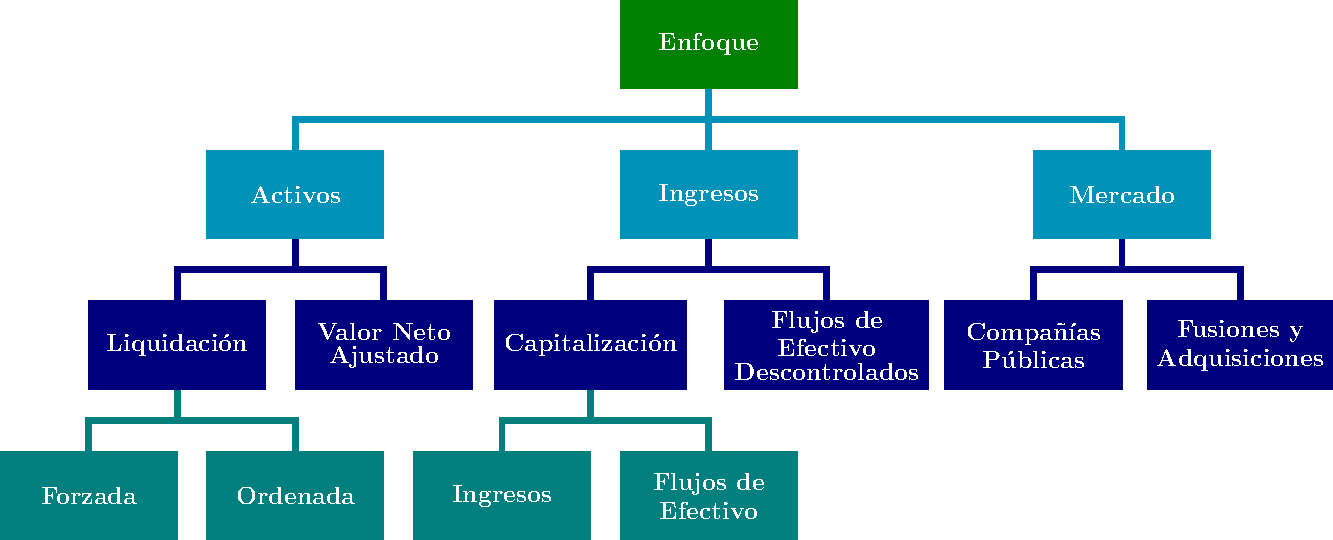
\includegraphics[width=14cm]{\rutaImagenes/enfoques_mas_utilizados}
\end{figure}


\subsubsection{Enfoque de Activos}

El enfoque de activos es una forma general de determinar el valor razonable del capital de una empresa, de un negocio, proyecto de inversi\'on, activo tangible o activo intangible; utilizando uno o m\'as m\'etodos basados en el valor de los activos y sus pasivos netos.\\[10pt]

En valuaci\'on de negocios, el enfoque de activos puede considerarse equivalente al enfoque de costos para otras disciplinas de valuaci\'on.\\[10pt]

Existen 2 m\'etodos generales en el enfoque de activos para la valuaci\'on de negocios:\\[10pt]

\textcolor{secundario}{M\'etodo de Valor en Libros Ajustado.} M\'etodo por el cual los activos y pasivos (incluyendo rubros fuera de balance, intangibles y pasivos contingentes) son ajustados a su valor de mercado.\\[10pt]

\textcolor{secundario}{M\'etodo de Capitalizaci\'on de Utilidades en Exceso.} Mediante este m\'etodo, se realiza una revaluaci\'on en conjunto de todos los activos y pasivos de la empresa. Este m\'etodo no se utiliza para determinar el valor total de un negocio, sino para determinar el valor del cr\'edito mercantil o de activos intangibles.\\[10pt]

Es importante distinguir entre la aplicaci\'on de un m\'etodo de valuaci\'on del enfoque de activos y el ``valor en libros''. Bajo cualquier est\'andar de valor, que el valor de mercado de un negocio o empresa sea igual a su valor en libros ser\'ia una coincidencia, o atender\'ia a circunstancias muy particulares de la entidad a valuar.

\subsubsection{Enfoque de Mercado}

En el enfoque de mercado se determina el valor razonable del capital de una empresa, de un negocio, proyecto de inversi\'on, activo tangible o activo intangible, al usar m\'etodos que comparan el activo valuado con activos similares.\\[10pt]

El negocio, acciones, activos tangibles o intangibles utilizados para la comparaci\'on, deben ser razonablemente similares al activo valuado. Los principales factores a considerar para determinar la comparabilidad incluyen:\\[10pt]

\begin{itemize}

\item Una similitud suficiente de las caracter\'isticas cuantitativas y cualitativas.
\item El monto y verificabilidad de la informaci\'on respecto del activo.
\item Si el precio del activo similar fue determinado en una operaci\'on entre partes independientes, es decir, en una venta de libre voluntad entre las partes.
\item Generalmente, las comparaciones se realizan mediante razones de valuaci\'on (m\'ultiplos); el c\'alculo y uso de dichas razones debiera proporcionar una referencia significativa respecto del valor del activo, considerando todos los factores relevantes.
\end{itemize}

Los m\'etodos del enfoque de mercado incluyen:\\[10pt]

\textcolor{secundario}{M\'etodo de Referencia de una Empresa P\'ublica}: M\'etodo por el cual se determinan m\'ultiplos de mercado de los precios de las acciones de compa\~n\'ias p\'ublicas (que coticen en una bolsa de valores) que tienen una l\'inea de negocio similar a la empresa valuada.\\[10pt]

\textcolor{secundario}{M\'etodo de Referencia de Transacciones}: M\'etodo por el cual se determinan m\'ultiplos de mercado de transacciones similares realizadas entre partes independientes.

\subsubsection{Enfoque de Ingresos}

El enfoque de ingresos es una forma general de determinar el valor razonable del capital de una empresa, de un negocio, activo, o de un activo intangible, utilizando uno o m\'as m\'etodos mediante los cuales los beneficios econ\'omicos son convertidos en valor.\\[10pt]

En el enfoque de ingresos, los beneficios anticipados se expresan en t\'erminos monetarios y pueden ser razonablemente representados por conceptos como dividendos o distribuciones, o varios tipos de utilidades o flujos de efectivo. \\[10pt]

Para estimar los beneficios anticipados se deben considerar elementos tales como la estructura de capital, el desempe\~no hist\'orico de la entidad, el entorno futuro en la industria, as\'i como factores econ\'omicos.\\[10pt]

Los beneficios anticipados se convierten en valor mediante procedimientos que consideran el crecimiento esperado y el momento en que se obtienen los beneficios, adem\'as del perfil de riesgo de los beneficios y el valor del dinero en el tiempo.\\[10pt]

Generalmente, la conversi\'on de beneficios anticipados en valor requiere de la determinaci\'on de un factor de capitalizaci\'on o una tasa de descuento. Para determinarlos, se deben considerar los niveles de las tasas de inter\'es, las tasas de retorno esperadas por los inversionistas en inversiones alternas, y las caracter\'isticas de riesgo espec\'ificas de los beneficios anticipados.\\